\RequirePackage{etex}

\documentclass[12pt,a4paper]{article}
\usepackage{hyperref}
\usepackage{amsthm}
\usepackage{amsfonts}
\usepackage{amsmath}
\usepackage{amssymb}
\usepackage{listings}
\usepackage{pgfcore}
\usepackage{hyperref}
\usepackage{tikz}
\usetikzlibrary{automata, positioning, arrows}

\tikzset{
    ->, % makes the edges directed
    >=stealth', % makes the arrow heads bold
    every state/.style={thick, fill=gray!10}, % sets the properties for each ’state’ node
    initial text=$ $, % sets the text that appears on the start arrow
}

\hypersetup{final}

\usepackage[
n, % o r lambda
advantage,
operators,
sets,
adversary,
landau,
probability,
notions,
logic,
ff,
mm,
primitives,
events,
complexity,
oracles,
asymptotics,
keys]{cryptocode}

\theoremstyle{definition}
\newtheorem{definition}{Definition}[section]

\newtheorem{theorem}{Theorem}[section]


\begin{document}


\title{\texttt{\detokenize{Lightning Pool:}} \\
    A Non-Custodial Channel Lease Marketplace}
\author{
    Olaoluwa Osuntokun \\ 
    \small{roasbeef@lightning.engineering}
    \and
    Conner Fromknecht \\
    \small{conner@lightning.engineering}
     \and
     Wilmer Paulino  \\
    \small{wilmer@lightning.engineering}
     \and
     Oliver Gugger \\
    \small{oliver@lightning.engineering}
     \and
     Johan Halseth \\
    \small{johan@lightning.engineering}
}

\date{\today}
\maketitle

\begin{abstract}

% The Lightning Network is an off-chain Layer 2 payment network built on the
% Bitcoin blockchain. As the network is fully collateralized, participants must
% commit capital to the network in the form of channels in order to use the
% network. 

In this paper we examine the core inbound liquidity bootstrapping problem the
Lightning Network faces, and frame it as a resource allocation problem to be
solved by application of market design and auction theory. We present Lightning
Pool, a non-custodial channel lease marketplace, implemented as a sealed-bid
frequent batched uniform clearing price auction which allows participants to
buy/sell capital obligations on the network. We call these capital obligations
\emph{channel leases}. A channel lease can be viewed as a cross between a
traditional fixed-income asset and an internet peering agreement. Channel
leases allow nodes on the network with idle capital to earn yield (based on a
derived \emph{per-block} interest rate) by selling a channel to an agent within
the marketplace, The duration of such a contract is enforced on-chain using
Bitcoin Script. We construct \textbf{Lightning Pool}, using a novel design for
constructing overlay applications on top of Bitcoin: a shadow chain. Shadow
chains allow users to remain in full custody of their funds at all times while
also participating in higher level cut-throughable applications. 

\end{abstract}

\section{Introduction}

\textbf{Lightning Network Bootstrapping Challenges}. The Lightning Network
(cite) is the largest deployed Layer 2 payment channel network (cite). A
payment channel network comprises of a series of individual payment channels,
which when strung together, enable rapid low-latency payments between
participants on the network. Due to the off-chain nature of these payments
(only the final summary hits the blockchain), the cost of payments on the LN
are typically much lower than an equivalent payment on the base blockchain
(cite). In order to be able to send funds on a network, a user must open a
payment channel (cite) to another participant on the network. Once the channel
has been opened, both participants are able to send/receive a nearly unbounded
number of payments off-chain, possibly never closing the channel on-chain to
delivery the contained funds. Similarly, in order to receive on the network, a
user requires \emph{another individual} to open a channel \emph{to} the
receiver. A participant can only send and receive up to the total amount of
Bitcoin in a channel committed by both parties. This allocation of capital by
one party in order to enable another party to receive funds on the network is
typically referred to as \emph{inbound liquidity} or \emph{inbound bandwidth}.
A would-be user of the network must somehow convince \emph{others} to allocate
capital towards them in order to receive funds on the network, the inbound
bandwidth problems remains a significant barrier to the adoption and
bootstrapping of the Lightning Network. 

\textbf{Routing Node Capital Requirements}.  In order to incentivize users to
commit capital to the network to help other users of the network send/receive
payments, each time a node forwards a payment successfully they receive a fee
dictated by themselves. As commonly implemented this fee has a fixed base
amount to be paid for all forward independent of payment size, and a fee rate
or proportional amount that must be paid for each millionth of a satoshi
forwarded (cite). We refer to nodes that join in order to facilitate payments
and collect forwarding fees: \emph{routing nodes}. In order to forward a
payment of size $N$ on the network, a routing node needs to have $N_{in} - F$
Bitcoin allocated \emph{towards} it as inbound bandwidth, and $N_{out}$ Bitcoin
allocated to another node as inbound bandwidth. The factor of $F$ is the fee
collected by the routing node, with the following constraint being met $F =
N_{out} - N_{in}$. Due to this requirement of having sufficient inbound
\emph{and} outbound bandwidth, even those nodes which exist solely to help
other nodes send/receive themselves must face the inbound bandwidth allocation
problem, the fundamental bootstrapping issue that the LN faces. 

\textbf{Market Design Resource Allocation Problems}. The field of market design
is a sub-field of economics which is concerned primarily with the efficient
allocation of scarce resources (cite). Within this sub-field, of interest is a
branch of market design concerned with instances wherein money is used to
govern the exchange of goods and services: auction design (cite). Auction
design can be used to effectively allocate scarce resources within a domain.
Common established examples of market design widely used today include:
emission of carbon credits, electricity markets, auctions for airpot slot
usage, and wireless spectrum auctions (cite) (cite) (cite). In each of these
examples, market design is used to allow more effective communication of
pricing information, resource allocation, and preference expressions (cite).
Our first insight is framing the solution to the inbound bandwidth
bootstrapping problem within the lense of market design. In the context of the
LN, the scarce resource we aim to more efficiently allocate is: inbound channel
bandwidth, which is commonly referred to as inbound liquidity. 

\textbf{LN Bootstrapping as Resource Allocation Problem}. In the absence of a
proper venue, those that need inbound capital to operate their Lightning
service are forced to solicit capital on various chat groups, forums, and also
Twitter. On the other side, those seeking to deploy capital in order to
facilitate network operation and gain routing fees must guess as to exactly
where their capital is most demanded. As node operators may not necessarily
know where their capital is most demanded, they risk opening channels where
they aren?t actually demanded, leading to poor resource utilization and capital
opportunity costs. It?s as if node operators are speculatively building roads
that no one will use (why isn?t my node forwarding?), and those seeking to
receive aren?t able to flag their service as an attractive destination to be
connected to internal network ?highways?. Lightning Pool solves this resource
allocation problem by creating a new auction that matches up those seeking to
deploy capital (open channels) to those that need these channels in order to
operate their Lightning service or business. With each executed batch, the
participants of the auction derive a \emph{per block} interest rate which is
effectively the current lease rate for capital on the Lightning Network. The
auctioneer or an independent agency is also able to provide Node Ratings to
participants of the network, which can be used to make more informed decisions
with respect to the \emph{quality} of the channel lease being purchased. (cite
predatory routing hi-jacking stuff)

\textbf{Channel Lease Marketplaces}. In this paper, we present Lightning Pool,
a non-custodial channel lease marketplace that draws on modern auction theory
to construct an auction that enables participants to buy/sell inbound channel
bandwidth. Participants of the marketplace buy/sell channel capital obligations
which we call a Lightning Channel Lease (LCL). An LCL is similar to a
traditional bond in that one party acquires capital form another for productive
usage, with the party parting with their capital being compensated for their
cost of capital. However as the funds within an LCL can only be used in the
Lightning Network for sending/receiving, an LCL is analogous to the creation of
a new virtual "road" within the LN connecting two destinations. Critically,
when one purchases an LCL the period of time those funds must be committed is
enforced on-chain using Bitcoin Script. As a result, buyers of inbound channel
bandwidth can be sure the capital will be committed for a set period of time.
The auction itself contains several sub-auctions for the exchange of particular
duration intervals expressed in blocks (similar to the various U.S Treasury
auctions (cite)). A non-trusted auctioneer facilities the market place by
accepting sealed-bid orders, clearing the market using a uniform clearing price
for each duration bucket, and finally executes a batch of contracts using a
single batch execution transaction that updates all involved accounts, and
delivers the purchased channels to all parties in an atomic manner. Lightning
Pool and the LCL solve the inbound bandwidth problem by allowing participants
on the network to effectively exchange pricing signals to determine exactly
\emph{where} in the network capital should be allocated. 


\textbf{Shadow Chains as an Application Framework}. Lightning Pool is the first
application built on top of Bitcoin that utilizes the \emph{Shadow Chain}
paradigm to construct an application-specific overlay system on top of existing
Bitcoin unspent transaction outputs (UTXOs). A user joins a shadow chain my
creating a special multi-sig based output using a public key of the target
shadow chain manager. Once a user has joined the shadow chain, proposed state
transitions are packaged up (in the form of a block) by the shadow chain
manager and proposed to each active participant. A shadow chain block updates
the application-state of all participants and is embedded within a normal
Bitcoin transaction. Depending on the application, a shadow-chain block may be
indistinguishable from a normal Bitcoin transaction. Shadow chains are able to
\emph{compress} state transitions \emph{off-chain} by employing a form of
multi-party transaction cut-through (cite). As participants of a shadow-chain
remain in custody of their funds at all times, complex fraud proofs or exit
games are unnecessary, significantly simplifying the implementation of a given
shadow chain. We note that the shadow chain itself is also of independent use. 

\subsection{Our Contributions}

In summary we make the following contributions: \begin{itemize} \item We
        propose a solution to the inbound bandwidth problem of the LN in the
        form of a market place to buy/sell inbound bandwidth obligations.
    \item We propose the Lightning Channel Lease, an inbound bandwidth
        obligation contract that pays a per-block interest rate to the seller
        from the buyer, and whose duration is enforced on-chain with Bitcoin
        Script.  \item We put forth the concept of a Node Rating agency for
        channel leases in order to provide marketplace participants with
        information about the \emph{quality} of a channel lease.  \item We
        construct a new system Lightning Pool, which is a non-custodial
        marketplace with off-chain order submission and on-chain batch
        execution that allow parties to exchange LCL contracts in an atomic
        manner.  \item We design a new Bitcoin application design framework,
the shadow chain, which is of independent use.  \end{itemize}
 
 
 \textbf{Organization}. Fill in final organization. 
 

\section{Preliminnaries}

not needed? 

% hash function
% signature
% random usage
% security param
% higher level transaction notation?


\section{Background}

In this section, we aim to introduce some necessary background which will be
built upon in later chapters to construct our solution. First, we'll describe
multi+hop payment channels and the Lightning Network as deployed today. Next,
we'll explore the nature of the inbound bandwidth bootstrapping problem the
Lightning Network faces today. Along the way we'll explain the dynamics of
routing nodes in the network, as they're a key component of the system. Next,
we introduce the field of market design, specifically the sub+field of auction
design to demonstrate how auction design can be used to solve resource
allocation problems in the real world. Next, we provide some brief background
on money markets in the traditional financial system, and how this relates to
our concept of channel leases. 

\subsection{Payment Channels \& the Lightning Network} 

\begin{center}
\textbf{Basic Payment Channels}
\end{center}

A payment channel (cite) in its simplest form (cite) is an on+chain 2+of~2
multi+sig output between to parties $A$ and $B$. One, or both parties deposit
funds into a script hash Bitcoin Script output constructed using two public
keys $P_{a}$ and $P_{b}$. The transaction which creates this multi-sig output
is referred to as the \emph{funding transaction}. Assuming a fix for
transaction ID level malleability (cite segwit) before broadcasting the funding
transaction, another transaction dubbed the \emph{commitment transaction} is
constructed given a series of paramaters by the two parties (cite bolt). The
commitment transaction spends the funding transaction and creates two new
outputs $D_{a}$ and $D_{b}$ which \emph{deliver} the current balance allocation
to both parties within the channel. Once the funding transaction is confirmed
and broadcasted both parties are able to rapidly update the balance of the
delivery outputs, $D_{a}$ and $D_{b}$ in order to make payments to one another. \\

\begin{center}
\textbf{Bi-Directional Payment Channels}
\end{center}

In order to safely make bi-directional payments between both parties, modern
channel designs also employ a \emph{commitment invalidation mechanism} (cite
paddy) to ensure that only the latest commitment transaction state can be
broadcasted and redeemed within the underlying blockchain. The most commonly
used commitment invalidation scheme is the \textbf{replace-by-revocation}
construct. In this construction, during channel negotiation, a security
parameter $T$ (which may be asymmetric for both parties) is negotiated. Using
this value $T$ which is typically expressed in blocks, a commitment transaction
state can only be fully redeemed by the broadcasting party after a period of
$T$ blocks has passed. During this interval the non-broadcasting party
$P_{defender}$ is able to provide the contested delivery output $D_{a_i}$ with
a valid witness $W_{r_n}$ which \emph{proves} that there exists a  \emph{newer}
state $n$ with $n > i$ which has been ratified by both parties. The exact
details of this construct are outside the scope of this party, but Bitcoin
Script and basic cryptography are used to allow a defending party to present an
objective statement of contract violation by the opposing party. \\

\begin{center}
\textbf{Hash Time Lock Contracts \& Multi-Hop Payments}
\end{center}


The final component of modern mult-hop payment channels is the Hash Time Locked
Contract, or the HTLC. The HTLC enables payments to travel over a \emph{series}
of payment channels, allowing set of interlinked payment channels to be
composed into a logical \emph{payment network}. An HTLC can be viewed as a
specific case of a time locked commit and reveal puzzle (cite ranjit?).
Loosely, an HTLC consists of four parameters: the public key of the sender
$P_{s}$, the public key of the receiver $P_{r}$, the payment amount expressed
in satoshis (cite) $A_{sat}$, a payment secret $r$ s.t $H(r) = h$, and an
absolute block timeout $T$. Given these parameters, a Bitcoin Script is set up
such that, the funds deposited in the script hash output can be redeemed by the
receiver $P_{r}$ via a public key signature by their public key and the reveal
of the payment pre-image $r$, or by the sender $P_{s}$ after the absolute
timeout $T$ has elapsed. This construct can be chained by several parties (up
to 20 in the modern Lightning Network (cite)) to create a multi-hop payment
within the network. For security properties, each party must ensure that their
outgoing hash lock puzzle's absolute timelock $T_o$ is offset from the incoming
absolute timelock $T_i$ by a value of $C_delta$. This value $C_{delta}$ is
commonly referred to as the CLTV delta (cite bolt). This value $C_{delta}$ is
an important security parameter, as if $C_{delta}$ blocks passes and the
outgoing hash lock isn't fully resolved, then a \emph{race condition} occurs as
the time out clauses of \emph{both} the incoming and outgoing hash locks have
expired. \\

\begin{center}
\textbf{Routing Nodes as Profit Seeking Capital Allocators}
\end{center}

Entities on the Lightning Network that exist primarily in order to collect fees
denominated in Bitcoin rewarded by successfully forwarding payments are
referred to as \emph{routing nodes}. A routing node commits capital to the
network within payment channels in order to be able to properly forward
payments in the network. (move much of that intro about the nodes here
insead?). As routing nodes incur an opportunity cost by committing the capital
to the network in place of other opportunities, they request a fee $F$ upon
completion of a successful payment forward. This fee $F = F_{base} +
F_{rate}*A_{sat}$ is comprised of two parts: a proportional amount (a rate) and
a fixed amount, which are both expressed in \emph{milli satoshis} which are
$1/1000$ of the base satoshi unit.

 Note that routing nodes are not compensated on an on going basis, and are not
 compensated for anything other than a completed payment. As a result, many
 routing nodes (cite aviv stuff) may be allocating capital in a non-productive
 manner as they've speculatively opened channels to areas of the network where
 no true transaction demand exists. If the Lightning Network was a physical
 transportation network, then it would be as if eager contractors started
 building roads to seemingly random destinations, only to find that those roads
 weren't actually demanded at all. This information asymmetry (where new
 channels are actually demanded) and the current inability for today's network
 participants to exchange these key demand signals lies as the crux of the
 bootstrapping problems of the Lightning Network. 


\subsection{Boostrapping Problems in the Lightning Network}

In this section, building on the background provided above, we aim to detail
the various bootstrapping problems that exist in the Lightning Network today.
These problems will serve motivation for our solution, the Channel Lease
Marketplace, and a specific instantiation of such a construct: Lightning Pool. 


\subsection{New Routing Node Boostrapping}

As the Lightning Network is a fully collaterized network, in order to
\emph{join} the system, a participant must commit capital in the form of
Bitcoin charged into payment channels on the network. Routing nodes however are
in a unique situation, as they need to both \emph{commit} their own capital to
the network, as well as \emph{solicit} committed capital from \emph{other}
routing nodes. This is due to the fact that in order to be able to forward a
payment of size $P_{sat}$, the routing node must first have $P_{sat_out}$
satoshis committed as \emph{outbound} payment bandwidth (to use for sending)
and $P_{sat_in}$ committed as \emph{inbound} payment bandwidth, with the
difference of the two amounts, $F= P_{sat_out} -  P_{sat_in}$ being collected
as a forwarding fee upon payment completion. This \emph{pair-wise} capital
commitment requirement is commonly cited as a major barrier to Lightning
Network adoption (cite), as well as why large "hubs" are inherently
economically inefficient (cite joseph SB montreal). 

A routing node faces two key questions when attempting to join the network in a
productive manner, while also attempting to optimize for \emph{capital}
efficiency: 

\begin{enumerate}
        \item \emph{Where} should I open channels to (thereby committing
            outbound capital) within the network in order to \emph{maximize}
            the velocity of my channels, and correspondingly my total fee
            revenue $F_r$? 

        \item \emph{How} can I attract \emph{other} routing nodes to commit
            capital to myself such that I can actually forward payments to earn
            \emph{any} revenue $F_r$?
\end{enumerate}

We argue that the above two questions, optimizing for capital efficiency and
velocity of committed channels, can only properly be addressed by the
\emph{existence} of a \emph{marketplace} which allows agents (routing nodes) to
communicate their preference using demand signals. Intuitively, a channel open
to an undesirable location (possibly over served) will have low channel
velocity $C_{v}$, and result in an overall lower total fee revenue $F_r$. In
order to maximize both $C_v$ and $F_fr$, a routing node should only open
channels to where they're \emph{most demanded}. If an agent is willing to pay
up to $P_premium$ Bitcoin for inbound bandwidth, the rationally, they must gain
more utility than the paid premium $P_premium$, as otherwise, such a
transaction would not be economically rationale. Thus, the existence of a
marketplace that allows routing nodes to efficiently commit their outbound
capital, as well as \emph{purchase} new inbound capital is a key component to
solving the boostrapping problem for routing nodes. 


\subsection{New Service Boostrapping}

If routing nodes are the the backbone or highway of the Lightning Network, then
so called Lightning Services, are the primary \emph{destinations} of a given
payment. For simplicity, we assume that at given Lightning Service is primarily
a payment \emph{sink}, in that it is primarily \emph{receiving} over the the
LN. In theory, it's possible for a service to send \emph{and} receiving,
resulting in a net-flow of zero, but today in the network, most flows are
uni-directional (cite), creating the need for on/off chain bridges such as
Lightning Loop (cite). 

\begin{center}
	\textbf{Demand for Incoming Bandwidth}
\end{center}

Focusing on the case of a Lightning Service that's pirimrilary a \emph{payment
sink}, on order to receive up to $N$ Bitcoin, the service requires $S_b$
Bitcoin to be committed as inbound capital, with $S_b > N$. Otherwise, assuming
only channel churn (cite bryan blog post), all inbound bandwidth will become
saturated, rendering a service unable to receive additional Bitcoin over the
LN. Therefore, the operative question a service needs to ask itself when
attempting to join the network is: 

\begin{itemize}
        \item How can I solicit enough inbound bandwidth within the network to
            be able to receive up to $S_b$ Bitcoin? 
\end{itemize}


\begin{center}
	\textbf{Preference for Quality of Bandwidth}
\end{center}

It's important to note, that as operating an \emph{valid} routing node on the
network requires a degree of skill and commitment (cite bryan blog post), some
routing nodes are able to provide a more \emph{effective} service than others.
As an example, imagine a routing node $Bob$, who has sufficient capital
committed to his not in both the inbound and outbound directions, but who is
chronically \emph{offline}. As a node must be \emph{online} in order to be able
to forward payments, any capital $C_Bob$ committed by $Bob$, can essentially be
considered dead weight. With this insight in mind, we revisit the bootstrapping
questions of the Lightning Service to also require a high \emph{quality of
service}:

\begin{itemize}
        \item How can I solicit enough \emph{high quality} inbound bandwidth
            within the network to be able to receive up to $S_b$ Bitcoin? 
\end{itemize}

\begin{center}
	\textbf{Time Committed Incoming bandwidth}
\end{center}


However, from the point of view of an active Lightning Service, just having
sufficient high quality inbound bandwidth may not be enough. Consider that a
high quality node $Carol$ may erroneously decide to commit capital elsewhere,
resulting in over all lower channel velocity $C_v$ for their channels. This
type of fair-weather behavior serves as a detriment to our Lightning Services,
as they're unable to properly plan for the future, as they don't know \emph{how
long} the inbound bandwidth will be available for receiving payments. As a
result, it's critical that the Lightning Service has a hard guarantee with
respect to \emph{how long} capital will be committed to their node. Taking this
new criteria into account, we further revisit our new service boostrapping
problem statement: 

\begin{itemize}
        \item How can I solicit enough \emph{high quality} inbound bandwidth
            within the network to be able to receive up to $S_b$ Bitcoin, that
            will be committed for \emph{at least} time $T_blocks$? 
\end{itemize} 

Summarizing, in addition to the existence of a marketplace for buying/selling
capital commitment obligations, a woiuld-be buyer requires some sort of
\emph{rating-system} to reduce information asymmetry (distinguish the good
nodes from the lemons), and also requires that any capital committed must be
committed for a period of $T_blocks$. These new requirements argue for the
existence of a Node Rating agency, as well as somewhere to ensure capital will
be committed for a set period of time in a trust-minimized manner. 


\subsection{End User Boostrapping}

Finally, we turn to the end users of the system. In our model, the end users of
the system are those that are frequently \emph{transacting}. If routing nodes
are the highways in our payment transportation network, the the Lightning
Services popular destinations, then users trigger \emph{payment flows} that
traverse the backbone created by routing nodes, to arrive at the Lightning
Services. Note that within our model, we permit end users to both send
\emph{and} receiver. Compared to boostrapping a new user to a Layer 1 system
such as the Bitcoin blockchain, boostrapping to a Layer 2 system like the
Lightning Network presents additional challenges. The core challenge is created
by the constraint that in order for a user to send $K_s$ Bitcoin, they also
need $K$ Bitcoin committed within the network. Similarly, in order to receive
up to $K_r$ Bitcoin, they need up to $K_r$ Bitcoin committed as inbound
bandwidth. 

From the perspective of attempting to achieve a similar level of
user-experience as a base Layer 1 system, the receiving constraint is the most
challenging. Notice that a user cannot simply download a Lightning wallet and
start receiving coins. Instead, they need to first solicit \emph{inbound}
capital to their node first. Many wallet providers such as Breez and Phoenix
have started to overcome this issue by committing capital to the users
themselves (cite). This can be see as a sort of customer acquisition cost: by
providing this inbound bandwidth to users, the wallet becomes more attractive
as it enables both sending and receiving. However, just receiving isn't enough,
a user also needs to be able to send \emph{and} receive. In addition to this
required symmetry, a typical user also has all the same quality of service, and
time committed capital requirement as well. 

With this background, we can phrase the end user boostrapping problem as
follows: 

\begin{itemize}
        \item How join the Lighting Network, in a manner that allows them to
            both send and receive to relevant destinations in the network? 
\end{itemize}


\subsection{Market Design \& Auction Theory}

In this section, we make a brief detour to the economic field of auction design
to examine how similar resource allocation problems can be solved by proper
market design in existing industries for both digital and physical goods. In
the modern age, market design and proper construction of corresponding
\emph{auctions} can be used to improve resource utilization and capital
efficiency (cite cramton
http://www.cramton.umd.edu/papers2010-2014/cramton-market-design.pdf) for a
given scare resource. Within a particular domain, several context-specific
design decisions are made to better optimize the resource allocation for all
participants involved. Common uses of auction design in the wild include
wireless spectrum auctions by the Federal Communications Comission (FCC)
(cite), package auctions for auctioning off takeoff and landing rights in
airpots (cite), real-time electricity markets (cite), and also carbon credits
(cite). Market design brides both theory and practice in order to solve
real-world resource allocation constraints (cite
http://www.cramton.umd.edu/papers2010-2014/cramton-market-design.pdf). 


A commonly used tool in the field of market design are \emph{auctions}.
Auctions allow agents to gather and exchange pricing signals in order to decide
who gets what goods, and at which price. The design of a proper auction for a
particular resource allocation problem has a vast design space. For example,
should a first or second price auction be used (cite)? How frequently should
the auction run? What \emph{type} of auction should be used? Should
participants be able to see the bids of other participants? And so on. 

Building off the series of boostrapping problems posed above, we turn to market
design as a tool to efficiently allocate our scare resource in question:
inbound payment bandwidth. Our problem-space is unique however in that as we're
dealing with the allocation of capital, there are inherent opportunity costs:
why should a routing node commit capital to the Lightning Network, compared to
some other asset that has a similar risk adjusted rate of return (cite)? In
this context, our end solution may take the form of a \emph{money market},
which is used by entities to trade short-term debt instruments. 

%add a sub-section on transportation systems?

\subsection{Money Markets \& Capital Leases} % Capital Markets & Channel Leases? 

In traditional financial markets, money markets are used to allow entities to
trade short term debt instruments. Examples of such instruments include U.S
Treasury Bills (cite), certificates of deposits (site), and repos or repurchase
agreements (cite). Capital markets on the other hand, are the long-term
analogue of money markets, in that they deal with longer time frames, and also
are more heavily traded on secondary markets with retail traders being more
involved. 

In the context of the Lightning Network, our concept of capital obligations
appears is similar to a bond in that we require a a prior period of time in
which the capital is allocated, but unlike a bond in that the committed funds
can only be used on the Lightning Network to provide a new type of service: the
\emph{propensity} to receive or send funds on the network. As a result, we
don't require funds in channels to be borrowed, instead they only need to be
\emph{leased} for a period of time. Also unlike bonds wherein it's possible for
the issuer of a bond to \emph{default}, thereby failing to repay the borrowed
money, in the context of the LN, there is \emph{no inherent default risk}.
Instead, arguably the concept of channel leases can be viewed as a risk free
rate of return (cite), in the context of Bitcoin, and specifically the
Lightning Network. 

The existence of a \emph{channel lease} serves to provide routing nodes with an
additional monetary incentive (in the form of a premium paid by the lessor of
the coins) to operate a routing node. As a result, we can modify the revenue
$R_c$ earned by a routing node within the context of a specific channel $C$,
for a period of $t$ blocks to be: 

\begin{equation}
R_c(t) = (P_c * t) + (F_c* P_{f_c}) % mak Pr[x] instead? 
\end{equation}

where $P_c$ is the current \emph{per-block} interest rate, and ($F_c *
P_{f_c}$) is the \emph{expected} routing fee revenue of the channel within that
interval \\ 

We reference an \emph{expectation} in fee revenue, as fees are effectively a
\emph{speculative} component of the routing revenue of a node. If a channel was
allocated to a node in high demand, one would expect the latter portion of the
question to possibly dominate the premium. If the opposite is the case, then a
routing node would derive most of its revenue from the yield earned by leasing
a channel. In this manner, the existence of a concept such as a channel lease,
actually serves to \emph{reduce} the variance of a routing nodes revenue,
similar to how joining a mining pool can reduce the variance of a hasher's
earnings (cite). 

Finally, we argue that the existence of a channel lease that pays a premium
based on a \emph{per-block} interest rate would result in a novel low-risk
yield-generating instrument for the greater Bitcoin network. Such a per-block
interest rate $r_{b_i}$ would serve to allow market participants to effectively
price the cost of capital on the Lightning Network. Assuming the existence of
varying durations ${D_1, ..., D_n}$ a \emph{yield} curve conveying the relative
short and long term interest rates of channel yields would be constructed. Such
an instrument would then potentially serve as the basis for higher level
structured products and derivates built on top of the base channel lease
instrument. 

%also add a solution overview here? 

\section{Bootstrapping Problems as Solved by CLM}

Prior to outlining our design for channel liquidity markets we seek to provide
a set of illuminating use-cases in order to demonstrate the need for such
markets on the Lightning Network. Each of these use cases are empirical
real-world problems related to the Lightning Network, and prior to the
publication of this document, no known solution has been presented. 

\subsection{Bootstrapping New Users via Sidecar Channels}

A common question posed concerning the Lightning Network goes something like:
Alice is new to Bitcoin entirely, how can she join the Lightning Network
without her, herself, making any new \emph{on-chain} Bitcoin transactions? It's
desirable to present a solution to such a use-case as on-boarding for on-chain
transaction is as simple as sending coins to a fresh address. In order for
off-chain payment channel networks to achieve wide-spread usage, a similar,
seamless on-boarding workflow must be created.

We frame the solution to this use-case in our model of channel liquidity
markets. In this case, Alice is a \emph{new} user to the network that requires
\emph{inbound} and \emph{outbound} liquidity. Without outbound liquidity, she's
unable to send to any other node on the network. Without inbound liquidity,
she's unable to receive any further payments on the network. We call our
solution "sidecar channels" they allow an acquaintance of Alice, let's call her
Carol, to engage in a protocol with an existing routing node on the network,
Bob, to provide \emph{both} inbound and outbound liquidity for Alice. Carol is
able to provide liquidity either with an off-chain, or on-chain payment. At the
end of the engagement, Carol has provided channel liquidity to Alice via Bob,
who himself is compensated accordingly for his role in the protocol. 

\subsection{Demand Fueled Routing Node Channel Selection}

A "routing" node on the Lightning Network is a node categorized as having a
persistent publicly reachable Internet address, a set of inbound channels from
leaf nodes, and one which seeks to actively facilitate payment flows on the
network in order to gain fee revenue using their existing liquidity as
bandwidth for these payment flows. A common question asked in the initial
bootrapping phase of the Lighting Network by node operators is: "where should I
open my channels to, such that they'll actually be routed through"? We posit
that channel liquidity markets are the answer to this question.

The channel liquidity market answer to this question is  supplementary to
autopilot \cite{autopilot} techniques of automated channel creation based on
static and dynamic graph signals. A key drawback of autopilot channel
establishment techniques are they for the most part, they're devoid of
\emph{economic} context. A particular location in the sub-graph may be "fit" or
attractive from a graph theoretic perspective, but may not lead to a high
velocity channel, as there was no inherent demand for a channel created at that
particular location. Using a CLM, a node operator can enter a targeted venue to
determine what the \emph{time value} of his liquidity is on the network. New
services such as exchanges or merchant on the network can bid for the node's
liquidity in order to serve their prospective customers, with the node earning
a small interest rate up-front for committing his liquidity in the first place
(scaled by the worst-case CSV delay). 

\subsection{Bootstrapping New Services to Lightning} 

Any new service that wishes join the Lightning Network faces the same problem:
"How can I incentivize nodes to create \emph{inbound} channels to me in order
to be able to accept payments?". CLM's provide an elegant solution. The
merchant/exchange/service uses their existing on-chain funds to enter the
liquidity market place in order to exchange their on-chain coins for off-chain
coins. Once the trade has been atomically executed, the merchant immediately
has usable inbound liquidity that can be used to accept payments from users. 

The merchant can then its prior market place exchange partners as
"introduction" points. As it's undesirable for all users to connect directly to
the merchant for payment connectivity, users can instead establish channels to
the prior swapping partners of the service. As the merchant acquires more
liquidity in the future, they further contribute to the path diversity and
strength of the network, allowing users to pay via several introduction points
using AMP \cite{amp}. 

\subsection{Cross-Chain Market Maker Liquidity Sourcing} 

As traders are becoming more aware of the counter-party risk of trading on
centralized exchanges, they look to non-custodial exchange venues. The
flexibility of channels on the Lightning Network appears to be a prime
candidate of such a venue: channels allow for non-custodial trading at similar
execution speeds to that of centralized exchanges. Additionally, channel based
non-custodial exchanges are not vulnerable to front-running tactics executed by
miners. Instead, the trade execution and even the prior trade history are
\emph{only} known to the participants a, providing a greater degree of
financial privacy. 

Once again, we encounter a bootstrapping issue. How is a market maker on a
payment channel based non-custodial exchange meant to gather an initial pool of
liquidity to service orders? We see CLMs as a natural solution. The market
maker can seek out liquidity of relevant trading pairs by purchasing inbound
channel liquidity, in addition to putting up its own outbound channel liquidity
to other market makers. A balanced distribution of liquidity amongst market
makers allows for new traders to participate in the exchange, knowing that
their flows are balanced, meaning they can receive as much as the can send via
the market maker, allowing them to instantly start to execute cross-chain
atomic swaps. 

\subsection{Instant Lightning Wallet User On Boarding}

Wallets commonly face the UX challenge of ensuring a user can receive funds as
soon as they set up a wallet. Some wallet providers have chosen to open new
inbound channels to users themselves. This gives users the inbound bandwidth
they need to receive, but can come at a high capital cost to the wallet
provider as they need to commit funds with a 1:1 ratio. The Pool allows them to
lower their customer acquisition costs, as they can pay only a percentage of
the funds to be allocated to a new user. Just like the merchant purchasing
inbound in the above segment, a wallet could pay 1k satoshis to have 1mm
satoshis be allocated to a user, instead of fronting the whole 1mm satoshis
themselves

\subsection{Variance Reduction in Routing Node Revenue}

Today routing node operators aim to join the network in order to facilitate the
transfer of payments as well as earn fees over time with successfully completed
payments. However, if a node isn?t regularly routing payments (thereby earning
a forwarding fee), then they aren?t compensated for the various (though minor)
risks they expose their capital to. With Pool, routing node operators are able
to ensure that they?re consistently compensated for their cost of capital. 

\section{The Channel Lease Marketplace} %definiation 

In this section, we present an overview of the Channel Lease Marketplace
architectural design. In section 6, we make a brief detour to define the
\emph{Shadow Chain} application frame work, before presenting a concrete
instantiation of a CLM, in the form of \textbf{Lightning Pool}. 

\subsection{High-Level Description}

First, we describe our solution at a high-level. Drawing heavily from existing
market auction design, we're interested specifically in double-call auctions
which allow both the buyer and the seller to buy/sell \emph{indivisible} units
of the good in question, which in this case is a channel lease. We then build
upon this base double-call auction by leveling the information playing field
(cite) by making all orders \emph{sealed-bid}. Rather than the auction being
cleared continually within a central-limit order book, we instead opt to
utilize a discrete interval frequent batched auction in order to mitigate
front-running and other undesirable aspects. Rather than participants paying
what they bid (commonly called a pay-as-you-bid auction (cite)(cite)), all
participants will instead pay the say \emph{uniform clearing price} (cite).
Finally, all operations that result from a sackful auction are batched and
committed in a \emph{single} atomic blockchain transaction.

\clearpage

\begin{figure}[!htb]

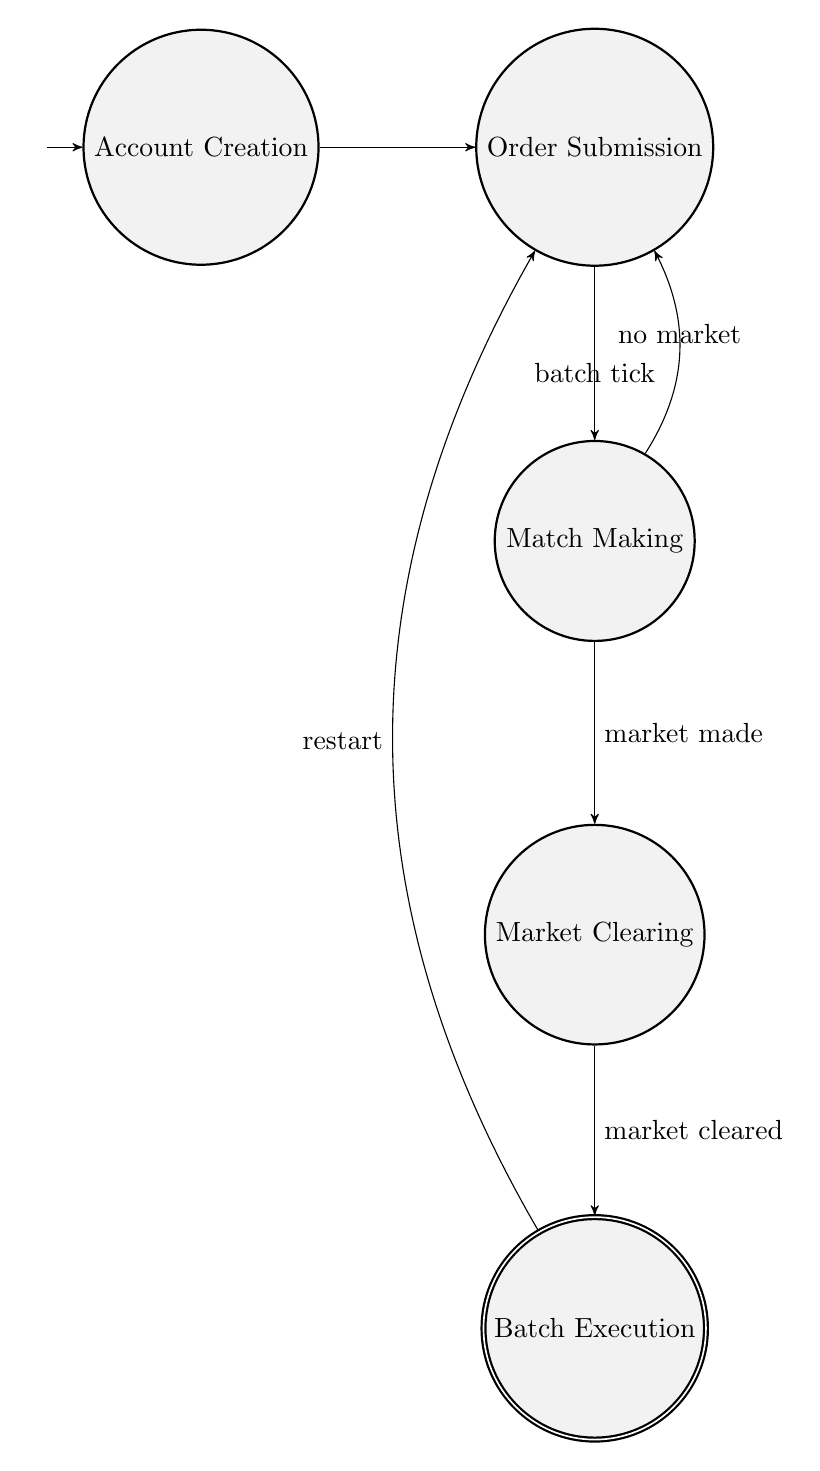
\begin{tikzpicture}[node distance=5cm,on grid,auto]
    \node[initial, state] (s0) {Account Creation};
    \node[state, right of=s0] (s1) {Order Submission};
    \node[state, below of=s1] (s2) {Match Making};
    \node[state, below of=s2] (s3) {Market Clearing};
    \node[state, accepting, below of=s3] (s4) {Batch Execution};

    \draw (s0) edge[right] node{} (s1)
          (s1) edge[below] node{batch tick} (s2)
          (s2) edge[bend right, above] node{no market} (s1)
          (s2) edge[right] node{market made} (s3)
          (s3) edge[right] node{market cleared} (s4)
          (s4) edge[bend left] node{restart} (s1);
\end{tikzpicture}

\caption{Auction State Machine}

\end{figure}


\begin{center}
    \textbf{Marketplace Auctioneer}
\end{center}

We assume the existence of a \emph{non-trusted} auctioneer $\Lambda$ that
publishes a master auctioneer key $A_{auction}$ ahead of time. The auction
itself is uniquely identified by $A_{auction}$ from the perspective of the
system due to the \emph{Shadow Chain} qualities of the system. The auctioneer
implements a non-custodial auction via \texttt{Marketplace Accounts} which use
a new unique key derived from $A_{auction}$ as the second public key in the
2-of-2 multi-sig. The auctioneer accepts and validates orders off-chain, aides
an agent in modifying their account before expiration, proposes a valid batch
to each of the agents matched in an instance of the auction, and produces a
batch execution transaction which modifies accounts appropriately, and creates
a series of corresponding channel leases.

\begin{center}
    \textbf{Account Creation}
\end{center}

Before being able to particiapte in the marketplace, we require that an agent
first create a \texttt{Marketplace Account}. A \texttt{Marketplace Account} is
a non-custodial account that forces an agent to commit capital in the form of
Bitcoin to the market for a period of time. As we require agents to fully back
all orders within an account, we eliminate a number of order spoofing vectors.
Additionally the time-locked non-custodial nature of the account ensures a user
is able to recover their funds fully without any additional on-chain
transactions (aside from the sweeping transaction).

\begin{center}
    \textbf{Marketplace Order Units}
\end{center}

We abstract over the base satoshi unit and define a \texttt{unit} from the PoV
of the marketplace which is the base unit in which all orders are expressed and
settled in. We assume that the value of a given \texttt{unit} is set such that
even a single lease of the smallest unit is still economical from the
perspective of the base blockchain and on-chain fees. All orders \emph{must} be
divisible by a whole unit, and the final clearing volume of a given batch is
also expressed in units.

\begin{center}
    \textbf{Order Submission}
\end{center}

Once an agent has created a valid \texttt{Marketplace Account}, they can enter
the order submission phase. It's important to note that this order submission
takes place \emph{off-chain}. Only the final execution of an auction batch
takes place on-chain. During the order submission phase, agents are free to
modify their accounts and orders. Only valid orders will be accepted to be
eligible for the next auction iteration.

\begin{center}
    \textbf{Market Clearing}
\end{center}

Every $\Upsilon$ minutes, the auctioneer attempts to \emph{clear} the marketplace.
An auction can be cleared if the lines of supply and demand cross such that at
least a single unit is bought/sold. As the market has no explicit closing time,
it's possible that during a market epoch, no market can be made. In the
scenario that a market can be made, then rather than each participant pay what
they bid, the auctioneer instead uses a single clearing price based on the
market's clearing price algorithm.

\begin{center}
    \textbf{Batch Execution}
\end{center}

Once a market has been cleared, we enter the batch execution phase. During this
phase, the auctioneer sends a batch proposal $\Pi$, which describes the
proposed market clearing structure. $\Pi$ may either be a plaintext description
of a valid clearing solution, or a more "argument" describing one.  Valid
batches are then bundled into a single \texttt{Batch Execution
Transaction} that updates all involved accounts, and creates any channel leases
bought/sold in the batch. After a period of time $\Upsilon$ has elapsed, the
market is restarted with any new orders and account being considered for market
clearing.

\subsection{Lightning Channel Leases}
\begin{center}
\textbf{Liquidity Maker \& Taker}
\end{center}

We begin by introducing the concept of a \texttt{Liquidity Taker}: 

\theoremstyle{definition}

\begin{definition}{(Liquidity Taker).} % call Lease instead? also define CLM earlier in the process? 
    A Liquidity Taker is an agent in a Channel Liquidity Market seeking to
    \emph{obtain} new \emph{inbound} channel liquidity of size $A_{sat}$ for a
    period of $T_{block}$ Bitcoin blocks. 
\end{definition}

A taker is prepared to either boostrap the inbound liquidity with their own
on-chain coins, or pay a \emph{premium} in order to receive a "lease" of
liquidity from another agent in the market. Takers populate the \emph{demand}
side of our market. They require new inbound liquidity in order to be able to
immediately receive payments on the network, or to better position themselves
as a routing node within the network. 

A natural companion to the Liquidity Taker agent within a \texttt{CLM} is the
\texttt{Liquidity Maker}: 

\theoremstyle{definition}
\begin{definition}{(Liquidity Maker).}

A Liquidity Taker is an agent in a Channel Liquidity Market seeking to earn
\emph{yield} by deploying up to $A_{sat}$ Bitcoin into the Lightning Network
for up to a period of $T_{block}$ Bitcoin blocks, earning a profit $\alpha$. 

\end{definition}

Notice that we utilize Bitcoin block-time rather than wall-clock (Median Past
Time (cite)) in these definitions, as we seek to enforce thee durations using
Bitcoin Script and using block-time rather than wall-clock time is more
objective compared to wall-clock time. 

The profit ($\alpha$) earned by a \texttt{Liquidity Maker} takes two forms: 
\begin{itemize}
   \item A one-time \emph{premium}, $R_{premium}$, commanded by the Maker which
       reflects the latent demand and time-value of regular coins vs "lifted
       coins" (coins placed in channels). 

   \item Ongoing reoccurring revenue, $F_c$,  in the form of forwarding fees
       earned by facilitating payments to their matched taker. 
\end{itemize} 


We argue that the existence of such Channel Liquidity Markets will increase the
\emph{efficiency} of capital deployed to a payment channel network by allowing
agents to signal the relative demand of lifted coins compared to non-lifted
coins. Additionally, such markets also allow an existing routing node on the
network to \emph{re-allocate} lifted coins from a low-velocity section of the
sub-graph, to one of higher velocity: 

\begin{theorem}[Channel velocity revenue] % remove? never used in a proof or anything 
Holding all channel liquidity equal, channels allocated to a higher velocity
section of the sub-graph will yield a higher $F_c$  than channel allocated to a
low-velocity section of the sub-graph. 
\end{theorem}

Intuitively, if each payment flow sourced at an incoming channel $C_i$ and sunk
at at outgoing channel $C_o$ pays and equal forwarding fee per flow, then for a
fixed unit of time, a higher velocity channel will result in higher total
revenue in a time slice. 

The role of Channel Liquidity Markets in a payment channel network is to reduce
information asymmetry by allowing agents to signal their preferences for lifted
coins vs non-lifted coins. The existence of \emph{venues} where these markets
can be carried out benefits the wider network by allowing agents to determine
where their liquidity if most demanded on the network. % remove?

\begin{center}
\textbf{Channel Leases}
\end{center}

With our two primary agents, defined, we now move on to the definition of a
Lightning Channel Lease: 

\begin{definition}{(Lightning Channel Lease).} 
    A Lightning Channel lease is defined as, $\Gamma = \{P_{T,} P_{M}, A_{sat},
    D_{block}, r_{i} \}$, where:
\end{definition}

\begin{itemize}
    \item $P_{T}$ is the \texttt{secp256k1} public key (cite) of the
\texttt{Liquidity Taker}, $P_{M}$ the public key for the \texttt{Liquidity
Maker}. 
    \item $A_{sat}$ is the total amount of Bitcoin within the contract.
    \item $D_{block}$ is the duration of the contract expressed in Blocks.
    \item $r_{i}$ is the per-block interest rate as discovered in the $i$th
    instance of the market.
\end{itemize}

Note that the premium $R_{P}$ as referenced above is parametrized in using the
\emph{lease duration} $D_{blocks}$: $R_{P}(D_{blocks}) = r_i * D_{blocks}$ as
we deal in simple, rather than compounding interest.  The duration of the
contract $D_{blocks}$ is of great interest as similar to U.S Treasury auctions,
a \emph{yield-curve} (cite) can be constructed based on the matched contents of
a given auction iteration. % mention t-bills


\subsection{Non-Custodial Auction Accounts}

In order to participate in the we require all participants to deposit their
trading balance into a Marketplace Account:

\theoremstyle{definition}
\begin{definition}{(Marketplace Account).}
A marketplace account is a \emph{non-custodial} account defined as, $\Psi =
\{K_{sat}, T_{blocks}, P_{acct}, \Omega_{nodes} \}$ where.
\end{definition}

\begin{itemize}
    \item $K_{sat}$ is the total amount of Bitcoin available within the account.
    \item $T_{blocks}$ is the absolute expiry height of the account. 
    \item $P_{acct}$ is a \texttt{secp256k1} public key  that \emph{uniqely} identifies the account.
    \item $\Omega_{nodes}$ is a set of Lighting Network nodes controlled by the account.
\end{itemize}

We stress that these accounts are \emph{non-custodial} in that after a period
of time $T_{blocks}$ the agent is able to freely remove the funds from their
account. Before this period has passed, an agent may require the aide of the
auctioneer to close, deposit, or withdraw funds from their account. In the case
of the \texttt{Liquidity Taker}, the funds within the account $K_{sat}$, must
be enough to pay for any desired premium, Conversely for the \texttt{Liquidity
Maker}, we require all funds they wish to lease out to be deposited into the
account. 

This structure, which forces all participants to fully commit all funds they
wish to use within the marketplace into a non-custodial account is similar to
the concept of Fidelity Bonds (cite). This structure has a number of desirable
properties including:

\begin{itemize} % what else? 
    \item \textbf{Order spoofing mitigation}: Within the CLM, as all orders
        must be "fully backed", it isn't possible to place a "fake" order that
        cannot be filled.

    \item \textbf{Time value opportunity cost}: By forcing all agents to
        suspend funds they wish to use within the market, those funds cannot be
        used elsewhere, thereby adding an implicit cost to joining the
        marketplace. 

    \item \textbf{Deterministic batch execution construction}: As we'll see in
        later sections, the existence of a fixed account for each agent
        simplified the clearing and execution process within the auction
        lifecycle. 

\end{itemize}

These accounts in the abstract may take many forms, but as we focus on Bitcoin,
as detailed in later sections, these accounts will take the form of a multi-sig
output, with one key belonging to the auctioneer. 

% define other operations for Deposit(), Withdraw(), Renew(), Close() or leave to the section below 

\subsection{Order Structure \& Verification}

With our channel lease contract and account structure defined, we now move on
to our order structure. As with any auction, orders are how the agents express
their \emph{preferences} with respect to what they wish to buy and sell.
Importantly, all orders within the market must be backed by a valid non-expired
account, and must carry an \emph{authentication tag} which prevents order
spoofing, and also ensure proper integrity of a given order once it has been
submitted

\begin{center}
\textbf{Order Structure}
\end{center}

We define an \texttt{Order} within the context of a \texttt{CLM} as follows: 

\theoremstyle{definition}
\begin{definition}{(Order).}
    An \texttt{Order} is a authenticated $n$-tuple: \\ $\Theta = \{O_{type}, K_{nonce},
    V_{ver}, P_{acct}, \Delta_{base}, \Delta_{aux}, T_{auth} \} $, where:

\end{definition}

\begin{itemize}
    \item $O_{type} \in \{\texttt{Ask}, \texttt{Bid}\}$ denotes if an order is
        an Ask or a Bid. In addition to the version, this may affect how the
        $\Delta_{aux}$ attribute is parsed.

    \item $K_{nonce}$ is an \emph{order nonce} which uniquely identifies this
        order, and is typically derived as $K_{nonce} = \sample
        \mathbb{Z}_{p}$.

    \item $V_{ver}$ is the \emph{version} of this order. As we'll see below,
        the version used as an upgrade mechanism, and is needed in order to
        parse any newly added fields, as well as compute the digest required to
        check the authentication tag attached to an order.

    \item $P_{acct}$ is the public key that uniquely identifies this account. 

    \item The set of base order details is: \\ $\Delta_{base} = \{
        \alpha_{rate}, A_{sat}, M_{pub}, L_{pub}, A_{addr}, C_{type},
    D_{blocks}, F_{chain} \}$, where:

    \begin{itemize}

        \item $\alpha_{rate}$ is the desired \emph{per-block} rate that the owner
            of the order wishes to buy/sell a channel lease at. Further below, this
            may be referred to ass the \texttt{BPY} or block percentage yield.

        \item $A_{sat}$ is the total contract size expressed in lease \emph{units}.
            Restricting orders to whole units simplifies preference matching within
            the system.

        \item $M_{pub}$ is the multi-sig public key to be used when creating
            the funding output (cite) of the tranction. % abstract out more?

        \item $L_{pub}$ is the identitiy public key (cite) of the Lightning
            Node that wishes to buy/sel lthis channel.

        \item $A_{addr}$ is the network address to be used to connect to the
            backing $L_{pub}$ to initiate the channel funding process if this
            order is matched. % too low level for this portion?

        \item $C_{type}$ is the \emph{type} of channel to be created if this
            order is matched.

        \item $D_{blocks}$ is the target \emph{lease duration} of the contract.

        \item $F_{chain_max}$ is the max chain fee expressed in $sat/byte$ that
            the own of said order is willing to pay within a batch.

    \end{itemize}

    \item The set of \emph{auxillary} details is implcitily defined by the
        order version $V_{ver}$.

    \item $T_{auth}$ is an authentication tag that allows the auctioneer, and
        other traders to validate the integrity and authenticity of the order.


\end{itemize}

An order allows a \texttt{Liquidity Taker} or a \texttt{Liquidity Maker} to
express their \emph{preference} with respect to what type of channel lease
they're looking to buy/sell.

\begin{center}
\textbf{Order Validation}
\end{center}

Returning back to our tag $T_{auth}$, we will now specify how such a tag is to
be computed, and verified. In the abstract, we require that the tagging scheme
is \seufcma secure (cite). Given this security requirement, we define
two polynomial-time algorithms: (\texttt{GenOrderTag}, \texttt{VerifyOrderTag})
with the following requirements:

\begin{itemize}
    \item \texttt{GenOrderTag($P_{acct_{priv}}$,$\Theta$)} $\rightarrow$ $T_{auth}$.
        Given an input of the private key that corresponds to the public key of
        an account, and the complete order details, a valid tag $T_{auth}$ is
        generated.

    \item \texttt{VerifyOrderTag($P_{acct}$,$\Theta$, $T_{auth}$)} $\rightarrow$ $b$.
        Given a public key of an account holder, a valid tag, and the order
        itself, \texttt{VerifyOrderTag} outputs $b=1$ if the tag is valid.
\end{itemize}

As we use a public-key based tagging technique, the validity of an order is
verifiable by any other active trader within the marketplace including the
auctioneer of the market place.


\subsection{Auction Design}

In this section, we describe the abstract definition of a \texttt{Channel
Liquidity Marketplace}, which addressee each of the issues presented in the
bootstrapping section of the background, by creating a new form of batched
auction which allows \texttt{Liquidity Takers}, and \texttt{Liquidity Makers}
to buy/sell Lightning Channel Leases in a non-custodial manner.

\subsubsection{Auction Specification}

In this section, we'll now specify the behavior and requirements of an using abstract
\texttt{Channel Liquidity Marketplace} instance. We define the expected
behavior and the client-facing interface of a \texttt{CLM} instance. A
\texttt{CLM} is a tuple of polynomial-time algorithms divided into five
distinct but related categories:
\begin{itemize}
    \item System Initialization: \texttt{SystemInit}
    \item Account Operations: (\texttt{NewAccount}, \texttt{ModifyAccount})
    \item Order Book Maintenance: (\texttt{SubmitOrder}, \texttt{CancelOrder})
    \item Market Clearing: (\texttt{MatchMake}, \texttt{MarketClearingPrice}, \texttt{ClearMarket})
    \item Batch Execution: (\texttt{ConstructBatch}, \texttt{ExecuteBatch})
\end{itemize}


With behavior and semantics as expressed below. \\

\begin{center}
    \textbf{System Initialization}
\end{center}

Before the market place can be used, we require it to be initialized by the
auctioneer. This initialization is a one-time process, and doesn't result in
any trapdoor or "toxic waste" material being produced: \\

\texttt{SystemInit($1^{\lambda}, \Upsilon_{min}$)} $\rightarrow$ ($P_{auction_p}$,
$P_{auction_s}, \Psi_{A}$). Denoting the security parameter as $\lambda$, the
    \texttt{SystemInit} algorithm takes as input the security parameter, and
    the batch interval $\Upsilon_{min}$ expressed in minutes, and outputs a
    public ($P_{auction_p}$) and private ($P_{auction_s}$) key pair for the
    auctioneer. The auctioneer's public key will be used as an parameter in
    algorithms related to account creation, modification, and batch execution.
    This algorithm also returns $\Psi_{A}$, which is a special account owned by
    the auctioneer that will be used to collect fees, and during batch
    construction.

\begin{center}
    \textbf{Account Operations}
\end{center}

In order to create an account, agents will need to interact with the auctioneer
itself. After account creation an account can freely be modified (close,
deposit, withdraw, etc) if the account isn't part of an active batch: \\

\texttt{NewAccount($1^{\lambda}, P_{auction_p}$)} $\rightarrow$ $\Psi$. The
\texttt{NewAccount} algorithm takes as input our security parameter, and the
auctioneer's public key, and outputs a new account for the new agent within the
marketplace. We require that all resulting accounts within the marketplace be
\emph{unique}. We permit a single logical agent to have multiple accounts. \\

\texttt{ModifyAccount($\Psi, P_{auction_p}$)} $\rightarrow$ $\Psi^\prime$. The % als needs the auctioneer's priv?
\texttt{ModifyAccount} algorithm takes an existing valid account $\Psi$ and the
auctioneer's public key and performs an account modification. An account
modification can either:
\begin{itemize}
    \item Deposit new coins into the account.
    \item Withdraw coins from the account.
    \item Close the account by removing all coins from the account.
\end{itemize}

Note that as each of these operations require an on-chain transaction, they can
freely be batched with other on-chain transactions, or even the transaction that
executes an auction's batch.

\begin{center}
    \textbf{Order Book Maintenance}
\end{center}

Once accounts in the marketplace are open, agents are able to submit orders
between batch epochs. The \emph{size} of all orders is expressed in units, and
as we mention below, we permit partial matches of an order. A partial match can
either update the order state in place, or require the agent to re-submit a new
valid tag for the modified order in the batch execution phase: \\

\texttt{SubmitOrder($\Theta, T_{auth}$)} $\rightarrow$ $b$. The
\texttt{SubmitOrder} algorithm takes as input a structurally sound order
$\Theta$, and its authentication tag $T_{auth}$ and outputs a bit $b$. The bit
$b=1$ if the order is valid according to market place rules, and the
\texttt{VerifyOrderTag} returns $b=1$ given the specified parameters. \\

\texttt{CancelOrder($\Theta, K_{nonce}^\prime$)} $\rightarrow$ $b$. The
\texttt{CancelOrder} given an existing order $\Theta$ and the \emph{opening} of
the $K_{nonce}$ commitment $K_{nonce}^\prime$ and returns $b=1$ if the
commitment opening is valid, and there exists an order identified by the base
$K_{nonce}$ value.

\begin{center}
    \textbf{Market Clearing}
\end{center}

Once all orders have been placed, and the batch interval of $\Upsilon$ has
elapsed, the auctioneer will attempt to clear the market using the following
algorithms: \\

\texttt{MatchMake($\{\Theta_0, \ldots, \Theta_n\}$)} $\rightarrow$
$\Phi_b = \{(\Theta_{b_0}, \Theta_{a_0}), \cdots, (\Theta_{b_n}, \Theta_{a_n})\}$. The
\texttt{MatchMake} algorithm takes as input the set of valid orders submitted
during the past batch interval and outputs a series of tuples which reflect
properly matched orders matched orders. $\Theta_a$ represents an order who's
$O_{type} = \texttt{Ask}$, while $\Theta_b$ represents an order who's $O_{type}
= \texttt{Bid}$. Note that since we allow \emph{partial} matches, a given order
may appear multiple times in the final match set. We require that a valid
implementation be able to perform proper \emph{multi-attribute} (cite) matching
due to the existence of the $\Delta_{aux}$ portion of an order's structure. \\

% state the specified constraints as a linear program??

 
\texttt{MarketClearingPrice($\Phi_b$)} $\rightarrow$ $c_{price}$. The
\texttt{MarketClearingPrice} algorithm accepts the set of orders matched by the
\texttt{MatchMake} algorithm and returns the \emph{market clearing price} of
the prior batch. The precise market clearing price algorithm is left as a free
parameter, with algorithms such as first-rejected-bid (cite) or
last-accepted-bid (cite) likely being used. Utilizing of a single market
clearing price is intended to promote fairness (cite) (all traders pay the same
price!) and also  \\

% give example of FRB and/or LAB here? 

% iamge of LAB clearing price here? 

\texttt{ClearMarket($\Psi_{A}, \Phi_b, \{\Psi_0, \dots, \Psi_n\}, c_{price}$)}
$\rightarrow$ $(\Psi_{A}^\prime, \{\Gamma_0, \dots, \Gamma_n\},
\{\Psi_{0}^\prime, \dots, \Psi_{n}^\prime\})$. The \texttt{ClearMarket}
algorithm takes as input a prior set of matched orders within a batch, the
auctioneer's account, the set of accounts involved in the bach, and the market
clearing price of a given batch and outputs: a set of channel leases to be
created by a batch and a set of updated accounts which represents the state of
the involved accounts post batch as well as an updated version of the
auctioneer's account which may have accrued any trading fees during market
clearing.

% cdots, ldots, or just dots -- need to make sure consistent everywhere

\begin{itemize}
    \item As shorthand, we use $\Delta_i$ to refer to a cleared batch (the set of
            resulting accounts after the updates have been made to produce the
            set of desired channel leases).
\end{itemize}

% takes the set of matched orders, and accounts, creates set of new accounts
% (diffs) 

\begin{center}
    \textbf{Batch Execution}
\end{center}

Once we've been able to make a market, and have the description of the
resulting market state (the accounts, and the channel leases to be created), we
can now move on to \emph{executing} the resulting batch. We use the following
algorithms to do so:  \\ 

\texttt{ConstructBatch($\Delta_i$)} $\rightarrow$ $B_{t_i}$. The
\texttt{ConstructBatch} algorithm takes a valid market clearing (which can be
seen as a delta on the auction state) and returns a valid transaction, which
\emph{atomically} executes the given batch on the blockchain. \\

\texttt{ExecuteBatch($B_{t_i}$)} $\rightarrow$ $b=$. The \texttt{ExecuteBatch}
algorithm takes a fully valid batch and attempts to commit it, by confirming
the transaction in the target base blockchain. Once the batch has been
confirmed, all operations contained within a batch are considered executed, and
can be used as inputs to additional iterations of the auction life cycle.

% have it return the batch ID? batch ID not shown any where there?

% have auction attribute section enumerating all from the blog post spill over
% portion?


\iffalse
shadow chain section: 
  * define as state machine that returns tate, then later define state in specific section to the the input of all the utxos and other state 
  
 ShadowChain:
    * Init() -> lambda params, w/e w/e 
    * state = InitState(auctioneerUtxo)
    * state = stateStep(state, stateDelta) -- a qurom needed to state step, 
    * propose set of updates to all 
        * for account := range accounts {
            proopse state 
         }
     * state_i = UpgradeState(state_i) 
     * state = {operatorKey, k_1, .., k_n}
     * state = stateFunc(state, proposal, executionEnv)
          * env can change off-chain, no need to on-chain upgrades, identified by hash/identifier 
     * order of execution func as way to impl soft-forks?  
     * state = coasalce(state_,1, ..., state_n) (transaction cut thru)
     * quorum = propose(masterKey, accounts) 
     * ^ then state func 
\fi

\section{The Shadowchain: A Bitcoin Overlay Application Framework}

In this section, we present the concept of a \texttt{Shadowchain}, a
non-custodial application overlay framework that we'll used to construct a
concrete instantiation of a \texttt{CLM}. We note that shadowchains may also be
of independent interest, as they're a novel way to layer more complex
interactions on top of the base Bitcoin blcockahin. We note that shadow chains
as we present them can be implemented on the base Bitcoin blockchain today
without any additional changes or enchainments. However, further extensions to
Bticoin such as non-interactive signature aggregation (cite) and covenants
(cite) can sever to dramatically increase the scalability traits of a
shadowchain.

\subsection{High-Level Description}

First, we provide a high-level description of the shadow chain application
framework. 

\textbf{The Shadowchain Usecase}. A shadowchain can be used to to implement
non-custodial smart contract systems on top of the base Bitcoin blockchain.
Typically one would opt for a shadowchain if the complexity of the state
transiting logic of the smart counteract system cannot be fully expressed using
the base Bitcoin Script.  Shadowchains allow an application designer to use the
Bitcoin blockchain for what it's best for: censorship resistant settlement,
pushing the more complex portions of the application (state, logic, etc)
\emph{off-chain}.

\textbf{Shadowchain Roles \& Lifted UTXOs}. A shadow chain has two primary
classes of agents: users, and the orchestrator.  The orchestrator defines the
state transition function of the shadowchain, a set of non-trusted
initialization parameters, and upgrade mechanisms. A user is able to join a
shadowchain by "lifting" their UTXOs \emph{into} the higher-level shadowchain.
The process of lifting (defined further below) entails the user placing funds
within a time-lock released multi-sig output between itself and the shadowchain
orchestrator. 

\textbf{Shadowchain Operation}. The shadowchain orchestrator accepts
transaction data from users, then periodically proposes a new \emph{shadowchain
block}. A shadowchain block takes as input the set of \texttt{Lifted UTXO}s
which accepted the latest block proposals, and produces a set of \emph{new}
UTXOs, which are the end state after the state transition function has been
evaluated. A shadowchain even permitted to use \emph{multiple} distinct state
transition functions. As the funds of an end user cannot move without both
multi-sig signatures, users are able to fully validate (possibly using
techniques such as zero knowledge proofs (cite shafi)) to validate that the
resulting UTXO state was properly derived from the known state transition
function.  Note that due to this structure complex "exit-games", or fraud
proofs are not required as as a user simply won't sign off on a fraudulent
state, and a user's UTXO is always manifested (in a base form) on the main
blockchain.

\textbf{Ephemeral Lifted UTXOs}. In the scenario that shadowchain operators
disappears, or is unresponsive, users are able convert their lifted UTXO into a
regular one, by spending their coins after the time-lock has expired. This
construct of an \emph{ephemeral} lifted UTXO has a number of desirable prop
ties on the application level, as the time-locked commitment of funds can serve
to mitigate a number of application-level issues such as spam or sybil
resistance.

\textbf{Shadowchain Cut-Through} As the evolution of a state transition
function happens \emph{off-chain}, it's possible to coalesce several distinct
shadowchain blocks into a single block which is the compositions of the
successive invocations of the state transition function. This technique is
similar to transaction cut-through (cite), but performed in a multi-party
setting. Leveraging this technique, as shadowchain operator can optimistically
treat the current latest shadowchain transaction in the mempool as an in-memory
data structure to be updated off-chain (via transaction replacement techniques
(cite)), with the state being "written to disk" once confirmed. As a result,
it's possible to commit several shadowchain states (possibly hundreds) in a
single logical Bitcoin transaction.

\textbf{Shadowchain Upgrades}. Finally, similar to the base blockchain, a
shadowchain can also be \emph{upgrade} in a forwards and backwards compatible
manner. In other words, it's possible for a shadowchain orchestrator to
\emph{soft-fork} the state transition logic by restricting a valid state
transition to enable new behavior. Notably, the operator can do this in a
de-synchronized manner as only those wishing to use features in the new state
transition function need to adhere to the new rules. Additionally, an operator
can opt to also introduces new backwards incompatible state transition funcs.
Due to the inherent batched nature of Bitcoin transaction, an operator can
commit multiple logical shadowchain blocks (with distinct state transition
functions) in a single atomic Bitcoin transaction.

To summarize, the shadowchain application framework is a novel technique for
constructing overlay applications on the base Bitcoin chain in a non-custodial
manner. Shadowchains avoid the complexity of fraud proofs and exit-games by
ensuring that the user has custody of their funds at all times and is able to
fully validate any proposed state transition. Shadowchains are able to compress
several logical state transitions into a single Bitcoin transaction using a
multi-party cut-through technique. An orchestrator of a shadowchain is also
able to upgrade the state transition logic on the fly, in a purely off-chain
manner.


\subsection{Comparison To Related Frameworks}

% do later?

\subsection{The Shadowchain Framework}

In this section, we present the abstract shadowchain application framework.
Applications are intended to use this framework, providing implementations of
specified virtual functions to fully specify and execute their application.

\subsubsection{Shadowchain Orchestrator}

First, we introduce the glue that keeps a shadowchain together, the
orchestrator:

\theoremstyle{definition}
\begin{definition}{(Orchestrator).} The \texttt{Orchestrator} is a non-trusted
    entity at the root of a shadowchain, parametrized by its long-term public
    key: $O_{chain} = P_{O}$. The duty of an \texttt{Orchestrator} is to
    propose new blocks (the result of a state transition) to the set of live
    \texttt{Lifted UTXO}s that make up the shadowchain.
\end{definition}

A given \texttt{Orchestrator} is a non-trusted entity, and can be uniquely
identified by its longer-term public key. The long-term public key $P_{O}$ can
also be used to uniquely identify a given shadowchain, similar to the Genesis
Block hash of a normal blockchain.

\subsubsection{Lifted UTXOs}

Next, we define the \texttt{Lifted UTXO} which is the representation of a
user's state within a given shadow chain:

\begin{definition}{(Lifted UTXO).} A \texttt{Lifted UTXO} is a tuple, 
    $ \phi = (A_{sat}, T_{expiry}, P_{u}, P_{o})$, where:
\end{definition}

\begin{itemize}
    \item $A_{sat}$ is the size of an \texttt{LO} (\texttt{Lifted UTXO})
        expressed in \emph{satoshis}.

    \item $T_{expiry}$ is the \emph{absolute} expiry height of the \texttt{LO},
        after-which the owner is able to unilaterally move the funds back to
        the "base" Bitcoin blockchain.

    \item $P_{u}$ is the public key of the end-user, which is $1/2$ of the
        public keys used in the public key script of the output which manifests
        this \texttt{LO} on the base blockchain.

    \item $P_{o}$ is the public key of the \texttt{Orchestrator}, typically
        derived from its base long-term key $P_O$. This key will be used as the
        other half of the multi-sig script of the on-chain manifestation of the
        \texttt{LO}.
\end{itemize}

% actually don't use LO here after all?

The construct of a \texttt{Lifted UTXO} is similar to the existing concept of a
Fidelity Bond (cite), yet with an application specific twist. The time-lock
release nature of the UTXO means a user can always recover funds if the
\texttt{Orchestrator} becomes unresponsive. In addition to this, a natural cost
in the form of chain fees is added which increases the barrier for potentially
malicious users to interact with the shadow chain.

\subsubsection{The Shadowchain}

In this section, we present the abstract definition of a shadow chain, building
upon the definition provided above. In addition to this, we describer the
typical Shadowchain life cycle using the aide of some additional helper
functions, which are also intended to be supplied by the core application logic
itself.

\begin{center}
    \textbf{Shadowchain Components}
\end{center}

First, we define the core components of the shadowchain. 

\begin{definition}{(Shadowchain).} An instantiation of a \texttt{Shadowchain}
    is defined as a tuple: $\Sigma = (U_{L}, U_{O}, \Delta, E_{exe},
    A_{T})$, where:
\end{definition}

\begin{itemize}
    \item $U_{L} = \{\phi_i, \cdots, \phi_n\}$ is the set of non-expired
        \texttt{Lifted UTXO}s observed by the Orchestrator.

    \item $U_{0}$ is the current UTXO Orchestrator, where they may accrue
        application level fees.

    \item $\Delta =  \{ \Delta_{F_0}, \cdots, \Delta_{F_n} \}$ is the set of
        current state transition functions.

    \item $E_{exe}$ is the abstract execution environment of the Shadowchain
        which all participants will use to verify the correctness of a proposed
        state transition.

    \item $A_{T}$ is the abstract form of the structure of the higher-level
        application's fundamental transaction.

\end{itemize}

\begin{center}
    \textbf{Shadowchain Algorithms}
\end{center}

Given the above components, we define the operation of a Shadowchain using a
series of polynomial-time algorithms segmented into the following logical
categories:

\begin{itemize}
    \item System Initialization: \texttt{InitChain}
    \item UTXO Management: (\texttt{LiftUTXO}, \texttt{ExitChain})
    \item Block Proposal \& Validation: (\texttt{ConstructBlock}, \texttt{ProposeBlock})
    \item Block Cut-Through: \texttt{CoalesceBlock}
    \item Chain Execution: \texttt{CommitBlock}
    \item Chain Upgrade: \texttt{UpgradeChain}
\end{itemize}

% also shadowchain definition: (utxos, operator, env, stateFuncs)

% definition of state transition function

% algorithm description

% shadowchain applicatin life cycle


\section{Lightning Pool: A Channel Liquidity Marketplace as a Shadow Chain}

tag of that order. This is done by concatenating each items of the order into
a single byte stream, and then generating a valid signature using our
\texttt{Sign} algorithm:

\procedureblock[syntaxhighlight=auto]{GenOrderTag($P_{acct}$, $\Theta$)}{
    b \gets K_{nonce} \| V_{ver} \| P_{acct} \| \Delta_{base} \concat \Delta_{aux} \\
    tag \gets Sign(P_{acct}, b) \\
    return tag
}

% code for validate order here in full later


For the sake of this section, we're only
interested in two algorithms within the context of such a scheme $\Sigma =
(Sign, Ver)$. Using these two algorithms, we now C
generation and verification algorithms.


Once the Maker has determined the two parmaters to the auction, he constructs a special \emph{auction} script which will allow him to auction off his liquidity to the bidder that pays the highest \emph{premium}. This script will allow him to enter the auction phase, where either the auction will timeout (providing him with a refund), or the auction is successful, leading to creation of a next channel on the network (a successful exchange). The (unoptimized) auction Script template is as follows: 
\begin{verbatim}
OP_IF
    <T> OP_CHECKLOCKTIMEVERIFY
    <maker refund key> 
    OP_CHECKSIG
OP_ELSE
    <maker multi-sig key> 2 OP_CHECKMULTISIG
OP_ENDIF
\end{verbatim}
 
 The first clause is the timeout clause, it allows the Maker to simply wait out an auction and obtain a refund if the market conditions are undesirable, or he wishes to start a new auction with a fresh set of coins. The role of the timeout clause is to show potential Takers that the Maker has \emph{skin in the game}: by sending his coins to a time-locked output he provides a strong signal to the marketplace of his willingness to participate. A valid witness to execute this clause is (omitting the witness script for brevity) 
\begin{verbatim}
<refund sig> <1>
\end{verbatim}

 
 
 The second clause is the auction \emph{execution} clause. This clause will be executed in the scenario that the Maker finds a Taker willing to pay the premium that he dictates. Notice that the multi-sig clause only specifies a \emph{single} key. We'll use this little-trick to bind the Taker to the channel at auction execution time. A valid witness to execute this clause is (omitting the witness script again for brevity):
 \begin{verbatim}
<taker sig> <maker sig> <2> <taker key> <nil>
\end{verbatim}

\section{Security Analysis}
\section{Future Directions}
\section{Related Work}
\section{Conclusion}

\section{Acknolwdgments}

\bibliographystyle{abbrv}
\bibliography{main}

\end{document}
This is never printed
